\documentclass[]{krantz}
\usepackage{lmodern}
\usepackage{amssymb,amsmath}
\usepackage{ifxetex,ifluatex}
\usepackage{fixltx2e} % provides \textsubscript
\ifnum 0\ifxetex 1\fi\ifluatex 1\fi=0 % if pdftex
  \usepackage[T1]{fontenc}
  \usepackage[utf8]{inputenc}
\else % if luatex or xelatex
  \ifxetex
    \usepackage{mathspec}
  \else
    \usepackage{fontspec}
  \fi
  \defaultfontfeatures{Ligatures=TeX,Scale=MatchLowercase}
\fi
% use upquote if available, for straight quotes in verbatim environments
\IfFileExists{upquote.sty}{\usepackage{upquote}}{}
% use microtype if available
\IfFileExists{microtype.sty}{%
\usepackage{microtype}
\UseMicrotypeSet[protrusion]{basicmath} % disable protrusion for tt fonts
}{}
\usepackage[margin=1in]{geometry}
\usepackage{hyperref}
\hypersetup{unicode=true,
            pdftitle={Spatial Data Science with R},
            pdfauthor={Edzer Pebesma and Roger Bivand},
            pdfborder={0 0 0},
            breaklinks=true}
\urlstyle{same}  % don't use monospace font for urls
\usepackage{natbib}
\bibliographystyle{apalike}
\usepackage{color}
\usepackage{fancyvrb}
\newcommand{\VerbBar}{|}
\newcommand{\VERB}{\Verb[commandchars=\\\{\}]}
\DefineVerbatimEnvironment{Highlighting}{Verbatim}{commandchars=\\\{\}}
% Add ',fontsize=\small' for more characters per line
\usepackage{framed}
\definecolor{shadecolor}{RGB}{248,248,248}
\newenvironment{Shaded}{\begin{snugshade}}{\end{snugshade}}
\newcommand{\KeywordTok}[1]{\textcolor[rgb]{0.13,0.29,0.53}{\textbf{#1}}}
\newcommand{\DataTypeTok}[1]{\textcolor[rgb]{0.13,0.29,0.53}{#1}}
\newcommand{\DecValTok}[1]{\textcolor[rgb]{0.00,0.00,0.81}{#1}}
\newcommand{\BaseNTok}[1]{\textcolor[rgb]{0.00,0.00,0.81}{#1}}
\newcommand{\FloatTok}[1]{\textcolor[rgb]{0.00,0.00,0.81}{#1}}
\newcommand{\ConstantTok}[1]{\textcolor[rgb]{0.00,0.00,0.00}{#1}}
\newcommand{\CharTok}[1]{\textcolor[rgb]{0.31,0.60,0.02}{#1}}
\newcommand{\SpecialCharTok}[1]{\textcolor[rgb]{0.00,0.00,0.00}{#1}}
\newcommand{\StringTok}[1]{\textcolor[rgb]{0.31,0.60,0.02}{#1}}
\newcommand{\VerbatimStringTok}[1]{\textcolor[rgb]{0.31,0.60,0.02}{#1}}
\newcommand{\SpecialStringTok}[1]{\textcolor[rgb]{0.31,0.60,0.02}{#1}}
\newcommand{\ImportTok}[1]{#1}
\newcommand{\CommentTok}[1]{\textcolor[rgb]{0.56,0.35,0.01}{\textit{#1}}}
\newcommand{\DocumentationTok}[1]{\textcolor[rgb]{0.56,0.35,0.01}{\textbf{\textit{#1}}}}
\newcommand{\AnnotationTok}[1]{\textcolor[rgb]{0.56,0.35,0.01}{\textbf{\textit{#1}}}}
\newcommand{\CommentVarTok}[1]{\textcolor[rgb]{0.56,0.35,0.01}{\textbf{\textit{#1}}}}
\newcommand{\OtherTok}[1]{\textcolor[rgb]{0.56,0.35,0.01}{#1}}
\newcommand{\FunctionTok}[1]{\textcolor[rgb]{0.00,0.00,0.00}{#1}}
\newcommand{\VariableTok}[1]{\textcolor[rgb]{0.00,0.00,0.00}{#1}}
\newcommand{\ControlFlowTok}[1]{\textcolor[rgb]{0.13,0.29,0.53}{\textbf{#1}}}
\newcommand{\OperatorTok}[1]{\textcolor[rgb]{0.81,0.36,0.00}{\textbf{#1}}}
\newcommand{\BuiltInTok}[1]{#1}
\newcommand{\ExtensionTok}[1]{#1}
\newcommand{\PreprocessorTok}[1]{\textcolor[rgb]{0.56,0.35,0.01}{\textit{#1}}}
\newcommand{\AttributeTok}[1]{\textcolor[rgb]{0.77,0.63,0.00}{#1}}
\newcommand{\RegionMarkerTok}[1]{#1}
\newcommand{\InformationTok}[1]{\textcolor[rgb]{0.56,0.35,0.01}{\textbf{\textit{#1}}}}
\newcommand{\WarningTok}[1]{\textcolor[rgb]{0.56,0.35,0.01}{\textbf{\textit{#1}}}}
\newcommand{\AlertTok}[1]{\textcolor[rgb]{0.94,0.16,0.16}{#1}}
\newcommand{\ErrorTok}[1]{\textcolor[rgb]{0.64,0.00,0.00}{\textbf{#1}}}
\newcommand{\NormalTok}[1]{#1}
\usepackage{longtable,booktabs}
\usepackage{graphicx,grffile}
\makeatletter
\def\maxwidth{\ifdim\Gin@nat@width>\linewidth\linewidth\else\Gin@nat@width\fi}
\def\maxheight{\ifdim\Gin@nat@height>\textheight\textheight\else\Gin@nat@height\fi}
\makeatother
% Scale images if necessary, so that they will not overflow the page
% margins by default, and it is still possible to overwrite the defaults
% using explicit options in \includegraphics[width, height, ...]{}
\setkeys{Gin}{width=\maxwidth,height=\maxheight,keepaspectratio}
\IfFileExists{parskip.sty}{%
\usepackage{parskip}
}{% else
\setlength{\parindent}{0pt}
\setlength{\parskip}{6pt plus 2pt minus 1pt}
}
\setlength{\emergencystretch}{3em}  % prevent overfull lines
\providecommand{\tightlist}{%
  \setlength{\itemsep}{0pt}\setlength{\parskip}{0pt}}
\setcounter{secnumdepth}{5}
% Redefines (sub)paragraphs to behave more like sections
\ifx\paragraph\undefined\else
\let\oldparagraph\paragraph
\renewcommand{\paragraph}[1]{\oldparagraph{#1}\mbox{}}
\fi
\ifx\subparagraph\undefined\else
\let\oldsubparagraph\subparagraph
\renewcommand{\subparagraph}[1]{\oldsubparagraph{#1}\mbox{}}
\fi

%%% Use protect on footnotes to avoid problems with footnotes in titles
\let\rmarkdownfootnote\footnote%
\def\footnote{\protect\rmarkdownfootnote}

%%% Change title format to be more compact
\usepackage{titling}

% Create subtitle command for use in maketitle
\newcommand{\subtitle}[1]{
  \posttitle{
    \begin{center}\large#1\end{center}
    }
}

\setlength{\droptitle}{-2em}
  \title{Spatial Data Science with R}
  \pretitle{\vspace{\droptitle}\centering\huge}
  \posttitle{\par}
  \author{Edzer Pebesma and Roger Bivand}
  \preauthor{\centering\large\emph}
  \postauthor{\par}
  \predate{\centering\large\emph}
  \postdate{\par}
  \date{2018-03-14}

\usepackage{booktabs}
\usepackage{amsthm}
\makeatletter
\def\thm@space@setup{%
  \thm@preskip=8pt plus 2pt minus 4pt
  \thm@postskip=\thm@preskip
}
\makeatother

\usepackage{amsthm}
\newtheorem{theorem}{Theorem}[section]
\newtheorem{lemma}{Lemma}[section]
\theoremstyle{definition}
\newtheorem{definition}{Definition}[section]
\newtheorem{corollary}{Corollary}[section]
\newtheorem{proposition}{Proposition}[section]
\theoremstyle{definition}
\newtheorem{example}{Example}[section]
\theoremstyle{definition}
\newtheorem{exercise}{Exercise}[section]
\theoremstyle{remark}
\newtheorem*{remark}{Remark}
\newtheorem*{solution}{Solution}
\begin{document}
\maketitle

{
\setcounter{tocdepth}{2}
\tableofcontents
}
\section{Preface}\label{preface}

\part{Spatial Data}\label{part-spatial-data}

\section{Hello, world!}\label{intro}

Let's create a map:

\begin{Shaded}
\begin{Highlighting}[]
\KeywordTok{library}\NormalTok{(tidyverse)}
\CommentTok{#> -- Attaching packages ---------------------------------- tidyverse 1.2.1 --}
\CommentTok{#> √ ggplot2 2.2.1.9000     √ purrr   0.2.4     }
\CommentTok{#> √ tibble  1.4.2          √ dplyr   0.7.4     }
\CommentTok{#> √ tidyr   0.8.0          √ stringr 1.3.0     }
\CommentTok{#> √ readr   1.1.1          √ forcats 0.2.0}
\CommentTok{#> -- Conflicts ------------------------------------- tidyverse_conflicts() --}
\CommentTok{#> x dplyr::filter() masks stats::filter()}
\CommentTok{#> x dplyr::lag()    masks stats::lag()}
\KeywordTok{library}\NormalTok{(sf)}
\CommentTok{#> Loading required package: methods}
\CommentTok{#> Linking to GEOS 3.5.1, GDAL 2.2.1, proj.4 4.9.3}
\KeywordTok{system.file}\NormalTok{(}\StringTok{"gpkg/nc.gpkg"}\NormalTok{, }\DataTypeTok{package=}\StringTok{"sf"}\NormalTok{) }\OperatorTok
\StringTok{    }\NormalTok{read_sf }\OperatorTok
\StringTok{    }\KeywordTok{st_transform}\NormalTok{(}\DecValTok{32119}\NormalTok{) }\OperatorTok
\StringTok{    }\KeywordTok{select}\NormalTok{(BIR74) }\OperatorTok
\StringTok{    }\KeywordTok{plot}\NormalTok{(}\DataTypeTok{graticule =} \OtherTok{TRUE}\NormalTok{, }\DataTypeTok{axes =} \OtherTok{TRUE}\NormalTok{)}
\end{Highlighting}
\end{Shaded}

\begin{center}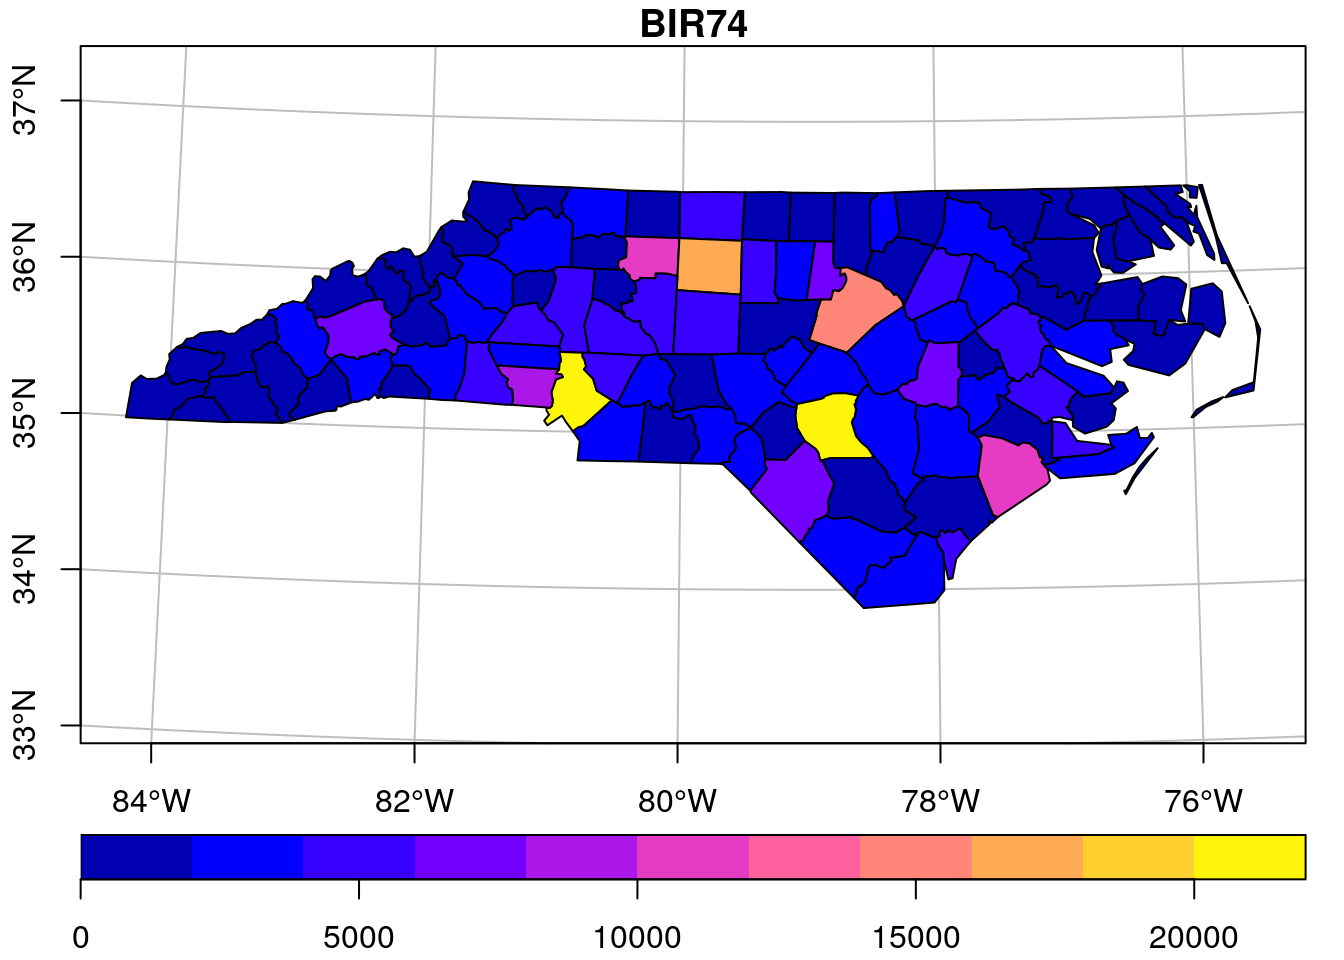
\includegraphics{sdsr_files/figure-latex/unnamed-chunk-3-1} \end{center}

A lot went on, here. We will describe the steps in detail. First, we
loaded two R packages:

\begin{Shaded}
\begin{Highlighting}[]
\KeywordTok{library}\NormalTok{(tidyverse)}
\KeywordTok{library}\NormalTok{(sf)}
\end{Highlighting}
\end{Shaded}

where \texttt{tidyverse} is needed for the tidyverse functions and
methods, and \texttt{sf} is needed for the spatial commands and spatial
tidyverse methods. The \texttt{\%\textgreater{}\%} (pipe) symbols should
be read as \emph{then}:

\begin{Shaded}
\begin{Highlighting}[]
\NormalTok{a }\OperatorTok\StringTok{ }\NormalTok{b }\OperatorTok\StringTok{ }\NormalTok{c }\OperatorTok\StringTok{ }\KeywordTok{d}\NormalTok{(}\DataTypeTok{n =} \DecValTok{10}\NormalTok{)}
\end{Highlighting}
\end{Shaded}

is simply another way of writing

\begin{Shaded}
\begin{Highlighting}[]
\KeywordTok{d}\NormalTok{(}\KeywordTok{c}\NormalTok{(}\KeywordTok{b}\NormalTok{(a)), }\DataTypeTok{n =} \DecValTok{10}\NormalTok{)}
\end{Highlighting}
\end{Shaded}

or alternatively

\begin{Shaded}
\begin{Highlighting}[]
\NormalTok{tmp1 <-}\StringTok{ }\KeywordTok{b}\NormalTok{(a)}
\NormalTok{tmp2 <-}\StringTok{ }\KeywordTok{c}\NormalTok{(tmp1)}
\NormalTok{tmp3 <-}\StringTok{ }\KeywordTok{d}\NormalTok{(tmp2, }\DataTypeTok{n =} \DecValTok{10}\NormalTok{)}
\end{Highlighting}
\end{Shaded}

but is easier to read, because we don't have to go from right to left,
and we don't have to choose names for intermediate results.

For the illustration we picked a data file that comes with \texttt{sf},
the location of which depends on your operating system:

\begin{Shaded}
\begin{Highlighting}[]
\NormalTok{(file <-}\StringTok{ }\KeywordTok{system.file}\NormalTok{(}\StringTok{"gpkg/nc.gpkg"}\NormalTok{, }\DataTypeTok{package=}\StringTok{"sf"}\NormalTok{))}
\CommentTok{#> [1] "/home/edzer/R/x86_64-pc-linux-gnu-library/3.4/sf/gpkg/nc.gpkg"}
\end{Highlighting}
\end{Shaded}

Parens around this expression are used to have the result not only
stored, but also printed.

Then, we read this file into R using \texttt{read\_sf}:

\begin{Shaded}
\begin{Highlighting}[]
\NormalTok{(nc <-}\StringTok{ }\KeywordTok{read_sf}\NormalTok{(file))}
\CommentTok{#> Simple feature collection with 100 features and 14 fields}
\CommentTok{#> geometry type:  MULTIPOLYGON}
\CommentTok{#> dimension:      XY}
\CommentTok{#> bbox:           xmin: -84.3 ymin: 33.9 xmax: -75.5 ymax: 36.6}
\CommentTok{#> epsg (SRID):    4267}
\CommentTok{#> proj4string:    +proj=longlat +datum=NAD27 +no_defs}
\CommentTok{#> # A tibble: 100 x 15}
\CommentTok{#>     AREA PERIMETER CNTY_ CNTY_ID NAME    FIPS  FIPSNO CRESS_ID BIR74 SID74}
\CommentTok{#>    <dbl>     <dbl> <dbl>   <dbl> <chr>   <chr>  <dbl>    <int> <dbl> <dbl>}
\CommentTok{#> 1 0.114       1.44  1825    1825 Ashe    37009  37009        5  1091  1.00}
\CommentTok{#> 2 0.0610      1.23  1827    1827 Allegh~ 37005  37005        3   487  0   }
\CommentTok{#> 3 0.143       1.63  1828    1828 Surry   37171  37171       86  3188  5.00}
\CommentTok{#> 4 0.0700      2.97  1831    1831 Currit~ 37053  37053       27   508  1.00}
\CommentTok{#> 5 0.153       2.21  1832    1832 Northa~ 37131  37131       66  1421  9.00}
\CommentTok{#> 6 0.0970      1.67  1833    1833 Hertfo~ 37091  37091       46  1452  7.00}
\CommentTok{#> # ... with 94 more rows, and 5 more variables: NWBIR74 <dbl>, BIR79 <dbl>,}
\CommentTok{#> #   SID79 <dbl>, NWBIR79 <dbl>, geom <MULTIPOLYGON [°]>}
\end{Highlighting}
\end{Shaded}

which creates a ``spatial tibble'':

\begin{Shaded}
\begin{Highlighting}[]
\KeywordTok{class}\NormalTok{(nc)}
\CommentTok{#> [1] "sf"         "tbl_df"     "tbl"        "data.frame"}
\end{Highlighting}
\end{Shaded}

This object is transformed into a new coordinate reference system (North
Carolina State Plane, with EPSG code 32119):

\begin{Shaded}
\begin{Highlighting}[]
\NormalTok{(nc}\FloatTok{.32119}\NormalTok{ <-}\StringTok{ }\KeywordTok{st_transform}\NormalTok{(nc, }\DecValTok{32119}\NormalTok{))}
\CommentTok{#> Simple feature collection with 100 features and 14 fields}
\CommentTok{#> geometry type:  MULTIPOLYGON}
\CommentTok{#> dimension:      XY}
\CommentTok{#> bbox:           xmin: 124000 ymin: 14700 xmax: 931000 ymax: 318000}
\CommentTok{#> epsg (SRID):    32119}
\CommentTok{#> proj4string:    +proj=lcc +lat_1=36.16666666666666 +lat_2=34.33333333333334 +lat_0=33.75 +lon_0=-79 +x_0=609601.22 +y_0=0 +ellps=GRS80 +towgs84=0,0,0,0,0,0,0 +units=m +no_defs}
\CommentTok{#> # A tibble: 100 x 15}
\CommentTok{#>     AREA PERIMETER CNTY_ CNTY_ID NAME    FIPS  FIPSNO CRESS_ID BIR74 SID74}
\CommentTok{#>    <dbl>     <dbl> <dbl>   <dbl> <chr>   <chr>  <dbl>    <int> <dbl> <dbl>}
\CommentTok{#> 1 0.114       1.44  1825    1825 Ashe    37009  37009        5  1091  1.00}
\CommentTok{#> 2 0.0610      1.23  1827    1827 Allegh~ 37005  37005        3   487  0   }
\CommentTok{#> 3 0.143       1.63  1828    1828 Surry   37171  37171       86  3188  5.00}
\CommentTok{#> 4 0.0700      2.97  1831    1831 Currit~ 37053  37053       27   508  1.00}
\CommentTok{#> 5 0.153       2.21  1832    1832 Northa~ 37131  37131       66  1421  9.00}
\CommentTok{#> 6 0.0970      1.67  1833    1833 Hertfo~ 37091  37091       46  1452  7.00}
\CommentTok{#> # ... with 94 more rows, and 5 more variables: NWBIR74 <dbl>, BIR79 <dbl>,}
\CommentTok{#> #   SID79 <dbl>, NWBIR79 <dbl>, geom <MULTIPOLYGON [m]>}
\end{Highlighting}
\end{Shaded}

and a single attribute column is selected

\begin{Shaded}
\begin{Highlighting}[]
\NormalTok{(nc.}\FloatTok{32119.}\NormalTok{bir74 <-}\StringTok{ }\KeywordTok{select}\NormalTok{(nc}\FloatTok{.32119}\NormalTok{, BIR74))}
\CommentTok{#> Simple feature collection with 100 features and 1 field}
\CommentTok{#> geometry type:  MULTIPOLYGON}
\CommentTok{#> dimension:      XY}
\CommentTok{#> bbox:           xmin: 124000 ymin: 14700 xmax: 931000 ymax: 318000}
\CommentTok{#> epsg (SRID):    32119}
\CommentTok{#> proj4string:    +proj=lcc +lat_1=36.16666666666666 +lat_2=34.33333333333334 +lat_0=33.75 +lon_0=-79 +x_0=609601.22 +y_0=0 +ellps=GRS80 +towgs84=0,0,0,0,0,0,0 +units=m +no_defs}
\CommentTok{#> # A tibble: 100 x 2}
\CommentTok{#>   BIR74                                                               geom}
\CommentTok{#>   <dbl>                                                 <MULTIPOLYGON [m]>}
\CommentTok{#> 1  1091 (((387345 278387, 381334 282774, 379438 282943, 373250 290553, 36~}
\CommentTok{#> 2   487 (((408602 292425, 408565 293985, 406643 296873, 406420 3e+05, 402~}
\CommentTok{#> 3  3188 (((478717 277490, 476936 278867, 471503 279173, 470806 281394, 46~}
\CommentTok{#> 4   508 (((878194 289128, 877381 291117, 875994 290881, 874941 292805, 87~}
\CommentTok{#> 5  1421 (((769835 277796, 768364 274842, 762616 274401, 763168 269009, 76~}
\CommentTok{#> 6  1452 (((812328 277876, 791158 277012, 789882 277579, 777724 277107, 76~}
\CommentTok{#> # ... with 94 more rows}
\end{Highlighting}
\end{Shaded}

Finally, the result is plotted, with the command:

\begin{Shaded}
\begin{Highlighting}[]
\KeywordTok{plot}\NormalTok{(nc.}\FloatTok{32119.}\NormalTok{bir74, }\DataTypeTok{graticule =} \OtherTok{TRUE}\NormalTok{, }\DataTypeTok{axes =} \OtherTok{TRUE}\NormalTok{)}
\end{Highlighting}
\end{Shaded}

\section{Spaces: 1, 2 and 3-dimensional, spherical, time, bounded
spaces}\label{spaces-1-2-and-3-dimensional-spherical-time-bounded-spaces}

discusses spaces

bounded: water, rivers, road networks

\section{Geometries}\label{geometries}

vertices, edges, lines, polygons, simple features; raster cells

\section{Vector/Raster}\label{vectorraster}

differences, correspondence; properties of rasters; arrays

\section{Geometric Manipulations}\label{geometric-manipulations}

discuss

\section{Attributes}\label{attributes}

discuss

\section{Reference Systems}\label{reference-systems}

Units of measure, reference systems, coordinate transformation and
conversion

\part{Maps}\label{part-maps}

\section{Plotting spatial data}\label{plotting-spatial-data}

Plotting of lines, symbols, polygons (choroplets; overlapping polygons),
rasters

using color

\section{Base Plot}\label{base-plot}

\section{ggplot2}\label{ggplot2}

\texttt{geom\_sf} examples; useful annotations and manipulations

\section{Interactive Maps}\label{interactive-maps}

base plot: identify, locator

leaflet, tmap, mapview

mapedit?

\part{Spatial Analysis}\label{part-spatial-analysis}

\section{Summarizing Geometries}\label{summarizing-geometries}

Properties: dimension, length, area, etc, if not earlier in Ch 3?

counts, density, intensity (units; meaningful)

\section{Point Pattern Analysis}\label{point-pattern-analysis}

Basics PP, beyond counting; basic steps in PPA

sf - spatstat interface; rasters;

\section{Manipulating attributes: summarise, aggregate, union,
sample}\label{manipulating-attributes-summarise-aggregate-union-sample}

\section{Units of measure revisited: attribute units, intensive and
extensive
variables}\label{units-of-measure-revisited-attribute-units-intensive-and-extensive-variables}

\section{Up- and Downscaling}\label{up--and-downscaling}

sampling

largest sub-geometry

area-weighted interpolation

\section{Spatial Interpolation and
geostatistics}\label{spatial-interpolation-and-geostatistics}

intro ; variograms; gstat (needs to be sf-ed)

\section{Area Data and Spatial
Correlation}\label{area-data-and-spatial-correlation}

spdep stuff

\section{Spatial Regression and
Autocorrelation}\label{spatial-regression-and-autocorrelation}

intro;

\section{Raster Modelling}\label{raster-modelling}

map algebra; ABM; SDM; Robert's book.

\part{Spatialtemporal
Analysis}\label{part-spatialtemporal-analysis}

\section{Array data: raster and vector data
cubes}\label{array-data-raster-and-vector-data-cubes}

\section{Movement data}\label{movement-data}

\section{Statistical modelling of spatiotemporal
data}\label{statistical-modelling-of-spatiotemporal-data}

\section{Scalability}\label{scalability}

\bibliography{book.bib,packages.bib}


\end{document}
